\documentclass[twocolumn]{article}

\usepackage[dvips]{graphics}
\usepackage{program}

\begin{document}

\title{Cassandra: Principles and Application}
\author{Dietrich Featherston\\
\small fthrstn2@illinois.edu\\
\small d@d2fn.com\\
\small \\
\small Department of Computer Science\\
\small University of Illinois at Urbana-Champaign
\small \\[-0.25in]} \date{}
\maketitle

\pagestyle{myheadings}
\markboth{D. Featherston}{Cassandra: Principles and Application}
\thispagestyle{empty}

\begin{abstract}
\noindent
Cassandra is a distributed database designed to be highly scalable both in terms of storage volume and request throughput while not being subject to any single point of failure. This paper presents an architectural overview of Cassandra and discusses how its design is founded in fundamental principles of distributed systems.  Merits of this design and practical use are given throughout this discussion.   Additionally, a project is supplied demonstrating how Cassandra can be leveraged to store and query high-volume, consumer-oriented airline flight data.
\end{abstract}

\section{Introduction}\label{s:intro}

Cassandra is a distributed key-value store capable of scaling to arbitrarily large sets with no single point of failure.   These data sets may span server nodes, racks, and even multiple data centers.  With many organizations measuring their structured data storage needs in terabytes and petabytes rather than gigabytes, technologies for working with information at scale are becoming more critical. As the scale of these systems grow to cover local and wide area networks, it is important that they continue functioning in the face of faults such as broken links, crashed routers, and failed nodes.  The failure of a single component in a distributed system is usually low, but the probability of failure at some point increases with direct proportion to the number of components.  Fault-tolerant, structured data stores for working with information at such a scale are in high demand.  Furthermore, the importance of data locality is growing as systems span large distances with many network hops.

% The failure of a single component in a distributed system is usually low, but the number of dependent parts increases the probability of failure at some point in the system with direct proportion to the number of dependent components.
% 
% \noindent
% Failure probability of a single component at time $t$
% \begin{equation}\label{singleFailure}
% P_i(t)
% \end{equation}
% 
% \noindent
% Failure probably somewhere within a distributed system with $n$ components at time $t$ given as the sum of the individual failure probabilities
% \begin{equation}\label{distributedFailure}
% P = \sum_{i=1}^n P_i(t)
% \end{equation}

Cassandra is designed to continue functioning in the face of component failure in a number of user configurable ways.  As we will see in sections \ref{s:cap} and \ref{s:consistency}, Cassandra enables high levels of system availability by compromising data consistency, but also allows the client to tune the extent of this tradeoff.  Data in Cassandra is optionally replicated onto $N$ different peers in its cluster while a gossip protocol ensures that each node maintains state regarding each of its peers.  This has the property of reducing the hard \emph{depends-on} relationship between any two nodes in the system which increases availability partition tolerance.

Cassandra's core design brings together the data model described in Google's Bigtable paper \cite{ref:bigtable} and the eventual consistency behavior of Amazon's Dynamo \cite{ref:dynamo}.  Cassandra, along with its remote Thrift API \cite{ref:thrift} (discussed in section \ref{s:api}), were initially developed by Facebook as a data platform to build many of their social services such as Inbox Search that scale to serve hundreds of millions of users \cite{ref:facebook}.

After being submitted to the Apache Software Foundation Incubator in 2009, Cassandra was accepted as a top-level Apache project in March of 2010 \cite{ref:apacheblog}.

In sections~\ref{s:cap} and \ref{s:consistency} we will see how Cassandra compensates for node failure and network partitioning.  More specifically, section~\ref{s:cap} discusses the fundamental characteristics distributed systems must sacrifice to gain resiliency to inevitable failures at sufficiently large scale.  Section \ref{s:datamodel} presents the basic data model Cassandra uses to store data and contrasts that model against traditional relational databases.  Section~\ref{s:dht} discusses distributed hash table (DHT) theory with section~\ref{s:storage} going into more detail on how Cassandra's implementation of a DHT enables fault tolerance and load balancing within the cluster.

Section~\ref{s:architecture} builds on previous sections with a deeper discussion of Cassandra's architecture. Section~\ref{s:consistency} discusses Cassandra's tunable consistency model for reading and writing data while section~\ref{s:replication} gives coverage to data replication within a cluster.  Section~\ref{s:elasticity} covers cluster growth and section~\ref{s:isolation} further contrasts the consistency and isolation guarantees of Cassandra against traditional ACID-compliant databases.  Finally, section~\ref{s:study} adds to the breadth of available case studies by showing how Cassandra can be used to model worldwide commercial airline traffic.

\subsection{CAP Theorem and PACELC}\label{s:cap}

Cassandra is one of many new data storage systems that makes up the \emph{NoSQL} movement.  NoSQL is a term often used to describe a class of non-relational databases that scale horizontally to very large data sets but do not in general make ACID guarantees.  NoSQL data stores vary widely in their offerings and what makes each unique.  In fact, some have observed that the entire movement is a way to group together fundamentally dissimilar systems based on what they do not have in common \cite{ref:datascience}.  However CAP, first conceived in 2000 by Eric Brewer and formalized into a theorem in 2002 by Nancy Lynch \cite{ref:brewer}, has become a useful model for describing the fundamental behavior of NoSQL systems.  A brief overview of this theorem is given, as well as a model which attempts to refine CAP as it relates to popular NoSQL systems. This overview will help support discussion of the tradeoffs made by the Cassandra data store in later sections.

The CAP Theorem states that it is impossible for a distributed service to be \emph{consistent}, \emph{available}, and \emph{partition-tolerant} at the same instant in time.  We define these terms as follows.

\begin{description}
\item[Consistency] means that all copies of data in the system appear the same to the outside observer at all times.
\item[Availability] means that the system as a whole continues to operate in spite of node failure.  For example, the hard drive in a server may fail.
\item[Partition-tolerance] requires that the system continue to operate in spite of arbitrary message loss.  Such an event may be caused by a crashed router or broken network link which prevents communication between groups of nodes.
\end{description}

Depending on the intended usage, the user of Cassandra can opt for Availability + Partition-tolerance or Consistency + Partition-tolerance.  These terms should not be interpreted as meaning the system is either available \emph{or} consistent, but that when there is a fault one or the other becomes more important for the system to maintain.  As a simple tool to grasp a complex subject, the CAP Theorem has rapidly become a popular model for understanding the necessary tradeoffs in distributed data systems.  However, this simplicity leaves room for potentially incorrect interpretation of the theorem.  Daniel Abadi of Yale University's Computer Science department has described a refining model referred to as PACELC which he uses to clarify some of the tradeoffs buried within the CAP Theorem. \cite{ref:pacelc}.

\begin{figure}[hp]
  \begin{center}
    \scalebox{0.53}{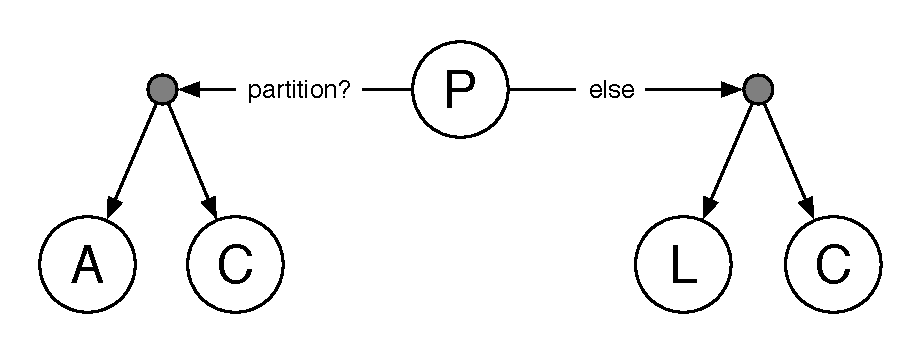
\includegraphics{pacelc.eps}}
  \end{center}
  \caption{PACELC Tradeoffs for Distributed Data Services}
  \label{fig:pacelc}
\end{figure}

Figure~\ref{fig:pacelc} diagrams the distributed data service tradespace as described by PACELC.  PACELC reformulates and clarifies CAP in a way that applies to many popular NoSQL systems--Cassandra included.  It states that when a system experiences partitioning $P$, it tends to require that tradeoffs be made between availability $A$ and consistency $C$.  Else $E$, under normal operation it must make tradeoffs between consistency $C$ and latency $L$.  This conjecture describes the real-world operation of Cassandra very well.  Under normal conditions, the user may make tradeoffs between consistency, sometimes referred to as \emph{replication-transparency}, and latency of operations.  However, when the system experiences partitioning, Cassandra must sacrifice consistency to remain available since write durability is impossible when a replica is present on a failed node.  The reasons behind these tradeoffs are made more clear in section~\ref{s:consistency}.

\section{Data Model}\label{s:datamodel}

Cassandra is a distributed key-value store. Unlike SQL queries which allow the client to express arbitrarily complex constraints and joining criteria, Cassandra only allows data to be queried by its key.  Additionally, indexes on non-key columns are not allowed and Cassandra does not include a join engine--the application must implement any necessary piecing together of related rows of data.  For this reason the Cassandra data modeler must choose keys that can be derived or discovered easily and ensure maintenance of referential integrity. Cassandra has adopted abstractions that closely align with the design of Bigtable \cite{ref:bigtable,ref:cwiki}.  While some of its terminology is similar to those familiar with relational databases, the reader should be careful not to think of how its abstractions map onto Cassandra.  The primary units of information in Cassandra parlance are outlined as follows.  This vernacular is used throughout the paper and is especially important to understanding the case study in section~\ref{s:study}.

\begin{description}
  \item[Column:] A \emph{column} is the atomic unit of information supported by Cassandra and is expressed in the form $name : value$.
  \item[Super Column:] \emph{Super columns} group together like columns with a common name and are useful for modeling complex data types such as addresses other simple data structures.
  \item[Row:] A \emph{Row} is the uniquely identifiable data in the system which groups together columns and super columns.  Every row in Cassandra is uniquely identifiable by its \emph{key}.  Row keys are important to understanding Cassandra's distributed hash table implementation.
  \item[Column Family:] A \emph{Column Family} is the unit of abstraction containing keyed rows which group together \emph{columns} and \emph{super columns} of highly structured data.  Column families have no defined schema of column names and types supported.  All logic regarding data interpretation stays within the application layer.  This is in stark contrast to the typical relational database which requires predefined column names and types.  All column names and values are stored as bytes of unlimited size and are usually interpreted as either UTF-8 strings or 64-bit long integer types.  In addition, columns within a column family can be sorted either by UTF-8-encoded name, long integer, timestamp, or using a custom algorithm provided by the application.  This sorting criteria is immutable and should be chosen wisely based on the semantics of the application.
  \item[Keyspace:] The \emph{Keyspace} is the top level unit of information in Cassandra.  Column families are subordinate to exactly one keyspace.  While variations exist, all queries for information in Cassandra take the general form $get(keyspace,column\_family,row\_key)$.
\end{description}

This data model provides the application with a great deal of freedom to evolve how information is structured with little ceremony surrounding schema design.  An exception to this rule is the definition of new keyspaces and column families which must be known at the time a Cassandra node starts \footnote[1]{This limitation is current as of the released version of Cassandra 0.6.3.  The current development version allows configuration of additional keyspaces and column families at runtime.}.  In addition, this configuration must be common to all nodes in a cluster meaning that changes to either will require an entire cluster to be rebooted.  However, once the appropriate configuration is in place, the only action required for an application to change the structure or schema of its data, is to start using the desired structure.  When applications require evolving their information structure in Cassandra, they typically implement a process of updating old rows as they are encountered.  This means applications may grow in complexity by maintaining additional code capable of interpreting this older data and migrating it to the new structure.  While in some circumstances this may be advantageous over maintaining a strictly typed data base, it underscores the importance of choosing a data model and key strategy carefully early in the design process.

\section{Distributed Hash Tables}\label{s:dht}

% Cassandra's data storage engine is driven by a distributed hash table.  In this section, the basics of distributed hash tables (DHTs) are discussed and in the next section (\ref{s:storage}) we discuss Cassandra's implementation of these principles.  These concepts are further built upon in section~\ref{s:architecture} as Cassandra's architecture is discussed in greater detail.

A distributed hash table is a strategy for decentralized, keyed data storage offering get and put operations: $get(key):value, put(key,value)$. Reliable decentralized lookup of data has been a popular research topic in the internet age.  Specifically, the area began to receive a great deal of attention during the rise and fall of Napster which maintained a listing file locations on a central server \cite{ref:beyondnap,ref:dht}.  Users would connect to the central server, browse for the data they want, and request that data over a point-to-point connection with the server containing the referenced data. However, there are a few problems with this approach. Any sufficiently large distributed system with a central coordinating node will experience bottlenecks at that node.  Large amount of strain in terms of processing power and bandwidth can arise at the central node which can make the entire system appear unavailable. DHTs offers a scalable alternative to the central server lookup which distributes lookup and storage over a number of peers with no central coordination required.

Any read or write operation on a DHT must locate the node containing information about the key. This is done through a system of \emph{key-based routing}.  Each node participating in a DHT contains a range of keys stored along with information about the range of keys available at 0 or more other nodes in the system.  Any node contacted for information regarding a key will forward that request to the next nearest node according to its lookup table. The more information each node maintains about its neighbors, the fewer hops required to get to the correct node.  While maintaining more state at each node means lower latency lookups due to a reduced number of hops, it also means nodes must exchange a greater amount of information about one other.  The tradeoff between lookup latency and internal \emph{gossip} between nodes is a fundamental driver behind DHT design. Many DHT systems such as \emph{Chord} exhibit $O(\log n)$ routing and interconnectedness complexity \cite{ref:chord,ref:onehop}. This is the case with many earlier DHT implementations which attempt at balance between network churn and lookup latency. Figure \ref{eq:dhtComplexity} shows some pairings of interconnectedness and lookup complexity of common DHT solutions \cite{ref:dht}.

\[
\begin{array}{ll}\label{eq:dhtComplexity}
  Connections & Number of Hops \\
  O(1) & O(n) \\
  O(\log n) & O(\log n) \\
  O(\sqrt n) & O(1)
\end{array}
\]

\subsection{Balanced Storage}\label{s:storage}

Cassandra's DHT implementation achieves $O(1)$ lookup complexity and is often referred to as a one-hop DHT.  This is a function of the gossip architecture in Cassandra which ensures each node eventually has state information for every other node. This includes the range of keys it is responsible for, a listing of other nodes and their availability, and other state information discussed in section~\ref{s:replication} \cite{ref:cgossip}.

Like other DHT implementations, nodes in a Cassandra cluster can be thought of as being arranged in a ring.  Servers are numbered sequentially around a ring with the highest numbered connecting back to the lowest numbered.  In Cassandra each server is assigned a unique \emph{token} which represents the range keys for which it will be responsible for. The the value of a token $t$ may be any integer such that $0 \le t \le 2^{127}$.  Keys in Cassandra may be a sequence of bytes or a 64-bit integer.  However, they are converted into the token domain using a consistent hashing algorithm.  MD5 hashing is used by default but an application may supply its own hashing function to achieve specific load balancing goals.  If a node $n$ in a token ring of size $N$ has token $t_n$ it is responsible for a key $k$ under the following conditions.

\begin{eqnarray*}
  0       <  &   n    &  <  N  \\
  t_{n-1} <  & md5(k) & \le t_n
\end{eqnarray*}

\noindent
Completing the token domain is the node with the lowest token value, $n = 0$, which is responsible for all keys $k$ matching the following criteria (\ref{eq:wrapwrange}).  This is often referred to as the \emph{wrapping range} since it captures all values at or below the lowest token as well as all values higher than the highest.

\begin{eqnarray}
  md5(k)  &   >   &  t_{N-1}  \nonumber\\
  md5(k)  &  \le  &  t_0      \label{eq:wrapwrange}
\end{eqnarray}

\noindent
As a result of employing the MD5 hashing algorithm for distributing responsibility for keys around the token ring, Cassandra achieves even distribution of data and processing responsibilities within the cluster.  This is due to the domain and range characteristics of the MD5 algorithm \cite{ref:md5}. Even when given similar but unique input, MD5 produces uniform output.  This even distribution of data within a cluster is essential to avoiding hotspots that could lead to overburdening a server's storage and capacity to handle queries.  The hashing algorithm applied to keys acts works to naturally load-balance a Cassandra cluster. 

\section{Architecture}\label{s:architecture}

Our discussion of DHTs is central to understanding Cassandra's architecture.  In the following sections we build on this understanding with discussions of how Cassandra implements reliable, decentralized data storage over DHT internals.

\subsection{Anatomy of Writes and Reads}\label{s:write}

To the user, all nodes in a Cassandra cluster appear identical. The fact that each node is responsible for managing a different part of the whole data set is transparent. While each node is responsible for only a subset of the data within the system, each node is  capable of servicing any user request to read from or write to a particular key.  Such requests are automatically proxied to the appropriate node by checking the key against the local replica of the token table.  Once a write request reaches the appropriate node, it is immediately written to the commit log which is an append-only, crash recovery file in durable storage.  The only I/O for which a client will be blocked is this append operation to the commit log which keeps write latency low.  A write request will not return a response until that write is durable in the commit log unless a consistency level of $ZERO$ is specified (see section~\ref{s:consistency} for details).  Simultaneously an in-memory data structure known as the \emph{memtable} is updated with this write.  Once this memtable (a term originating from the Bigtable paper \cite{ref:bigtable}) reaches a certain size it too is periodically flushed to durable storage known as a \emph{SSTable}.

Reads are much more I/O intensive than writes and typically incur higher latency.  Reads for a key at one of the replica nodes will first search the memcache for any requested column.  Any SSTables will also be searched.  Because the constituent columns for a key may be distributed among multiple SSTables, each SSTable includes an index to help locate those columns. As the number of keys stored at a node increases, so do the number of SSTables.  To help keep read latency under control, SSTables are periodically consolidated.

\subsection{Replication}\label{s:replication}

As discussed in sections \ref{s:dht} and \ref{s:storage}, Cassandra's storage engine implements a MD5-keyed distributed hash table to evenly distribute data across the cluster.  The DHT itself does not provide for fault-tolerance however since its design only accounts for a single node at which information regarding a key resides.  To allow keys to be read and written even when a responsible node has failed, Cassandra will keep $N$ copies distributed within the cluster.  $N$ is also known as the \emph{replication factor} and is configurable by the user.

The hashing function provides a lookup to the server primarily responsible for maintaining the row for a key.  However each node keeps a listing of $N-1$ alternate servers where it will maintain additional copies.  This listing is part of the information gossiped to every other node as described in sections \ref{s:storage} and \ref{s:elasticity}. When a live node in the cluster is contacted to read or write information regarding a key, it will consult the nearest copy if the primary node for that key is not available.  Higher values of $N$ contribute to availability and partition tolerance but at the expense of read-consistency of the replicas.

Cassandra provides two basic strategies for determining which node(s) should hold replicas for a each token. Each strategy is provided both the logical topology (token ring ordering) and physical layout (IP addresses) of the cluster.  For each token in the ring, the replication strategy returns $N-1$ alternate endpoints.

\begin{description}
  \item[Rack unaware] is the default strategy used by Cassandra and ignores the physical cluster topology.  This option begins at the primary node for a token and returns the endpoints of the next $N-1$ nodes in the token ring.
  \item[Rack aware strategy] attempts to improve availability by strategically placing replicas in different racks and data centers.  This design allows the system to continue operating in spite of a rack or whole data center being unavailable.  Nodes are assumed to be in different data centers if the second octet of their IPs differ and in different racks if the third octet differs.  This replication strategy attempts to find a single node in a separate data center, another on a different rack within the same data center, and finds the remaining $N-1$ endpoints using the rack unaware strategy. 
\end{description}

Users may also implement their own replica placement strategy to meet the specific needs of the system.  For example, a strategy may take physical node geography, network latency, or other specific characteristics into account.  The ability to tailor replica placement is an important part of architecting a sufficiently large Cassandra cluster, but by targeting replicas for certain nodes it is possible to introduce unwanted patterns into the distribution of data.  While this may be perfectly desirable in many cases, it is important to understand whether or not a given replica strategy will infect the cluster with unwanted hotspots of activity.

\subsection{Consistency}\label{s:consistency}

Cassandra is often communicated as being an eventually consistent data store.  While this is true for most cases in which Cassandra is suitable, in reality Cassandra allows the user to make tradeoffs between consistency and latency.  It does so by requiring that clients specify a desired consistency level--$ZERO$, $ONE$, $QUORUM$, $ALL$, or $ANY$ with each read or write operation.  Use of these consistency levels should be tuned in order to strike the appropriate balance between consistency and latency for the application.  In addition to reduced latency, lowering consistency requirements means that read and write services remain more highly available in the event of a network partition.

A consistency level of $ZERO$ indicates that a write should be processed completely asynchronously to the client.  This gives no consistency guarantee but offers the lowest possible latency.  This mode must only be used when the write operation can happen at most once and consistency is unimportant since there is no guarantee that write will be durable and ever seen by another read operation.  A consistency level of $ONE$ means that the write request won't return until at least one server where the key is stored has written the new data to its commit log.  If no member of the replica group for applicable token is available, the write fails.  Even if the server crashes immediately following this operation, the new data is guaranteed to eventually turn up for all reads after being brought back online. A consistency level of $ALL$ means that a write will fail unless all replicas are updated durably.  $QUORUM$ requires that $\frac{N}{2}+1$ servers must have durable copies where $N$ is the number of replicas.

A write consistency of $ANY$ has special properties that provide for even higher availability at the expense of consistency.  In this consistency mode Cassandra nodes can perform what is known as \emph{hinted handoff}.  When a write request is sent to a node in the cluster, if that node isn't responsible for the key of the write, then the request is transparently proxied to a replica for that token.  In the other synchronous write consistency modes $ONE$, $QUORUM$, and $ALL$, writes must be committed to durable storage at a node responsible for managing that key.  Hinted handoff allows writes to succeed without blocking the client pending handoff to a replica.  The fist node contacted, even if it is not a replica for that token, will maintain a hint and asynchronously ensure that the write eventually gets to a correct replica node.

Reads on the other hand require coordination among the same number of replicas but have some unique properties.  First, consistency modes of $ZERO$ and $ANY$ are special and only apply to writes.  The remaining consistency levels $ONE$, $QUORUM$, $ALL$, simply indicate the number of replicas that must be consulted during a read.  In all cases, if any replicas are in conflict the most recent is returned to the client.  In addition, any copies that are in conflict are repaired at the time of the read.  This is known in Cassandra parlance as \emph{read-repair}.  Whether this read-repair happens synchronously with the caller or asynchronously depends on the stringency of the consistency level specified.  If the specified number of replicas cannot be contacted, the read fails without fails based on the static quorum rules of the system.

Understanding how to tune the consistency of each read and write operation, we can now better understand how to balance between consistency and the combination of latency and fault-tolerance.  To achieve the lowest latency operations, the most lenient consistency levels may be chosen for reads and writes. If $R$ is given as the number of replicas consulted during a read, and $W$ as the number consulted during a write, Cassandra can be made fully consistent under the following condition.  Note that this is consistent with basic replication theory.

\begin{equation}\label{eq:consistency}
  R + W > N
\end{equation}

$QUORUM$ on reads and writes meets that requirement and is a common starting position which provides consistency without inhibiting performance or fault-tolerance.  If an application is more read or write heavy, then the consistency level can be tuned for that performance profile while maintaining total consistency as long as $R + W > N$.  If lower latency is required after exploring these options, one may choose $R + W <= N$.

As of this writing, Cassandra does not support the notion of a \emph{dynamic quorum} in which new quorum criteria are selected when the cluster is partitioned into two or more separate parts unable to communicate with one another \cite{ref:source,ref:cwiki}.  If a partition occurs that prevents the specified number of replicas from being consulted for either a read or write operation that operation will fail until the partition is repaired \cite{ref:cdk}.

\subsection{Isolation and Atomicity}\label{s:isolation}

It is important to mention that for many reliable data-intensive applications such as online banking or auction sites, there are portions of functionality for which consistency is only one important factor.  Factors such as atomicity of operations and isolation from other client updates can be critical in many cases and are often encapsulated within a transaction construct for relational databases.  In Cassandra there is no way to achieve isolation from other clients working on the same data.  Some atomicity is offered, but it is limited in scope.  Cassandra guarantees a reads or writes for a key within a single column family are always atomic.  There is no notion of a check-and-set operation that executes atomically and batch updates within a column family for multiple keys are not guaranteed atomicity \cite{ref:cwiki}.  Application designers choosing a data store should consider these criteria carefully against their requirements while selecting a data store.  In some cases applications designers may choose to put some subset of data that should be subject to ACID guarantees in a transactional relational database while some other data resides in a data store like Cassandra.

\newpage
\subsection{Elastic Storage}\label{s:elasticity}

Up to this point, discussion has focused on Cassandra's behavior in the context of a statically defined group of nodes.  However one of the attractions of Cassandra is that it allows scaling to arbitrarily large data sets without rethinking the fundamental approach to storage.  Specifically, hardware requirements and costs scale linearly with storage requirements.  Cassandra clusters scale through the addition of new servers rather than requiring the purchase of ever more powerful servers.  This is often referred to as horizontal versus vertical scaling.  To understand how a cluster can grow or shrink over time, we will revisit the topic of distributed hash tables as implemented by Cassandra.  Recall that nodes are arranged in a logical ring where each node is responsible for a range of keys as mapped to the token domain using consistent hashing.

The process of introducing a new node into a Cassandra cluster is referred to as \emph{bootstrapping} and is usually accomplished in one of two ways.  The first is to configure the node to bootstrap itself to a particular token which dictates its placement within the ring.  When a token is chosen specifically, some data from the node with the next highest token will begin migration to this node.  Figure~\ref{fig:bootstrap} shows a new node $t_{n\prime}$ being bootstrapped to a token between $t_{n-1}$ and $t_n$.

\begin{figure}[hp]
  \begin{center}
    \scalebox{0.5}{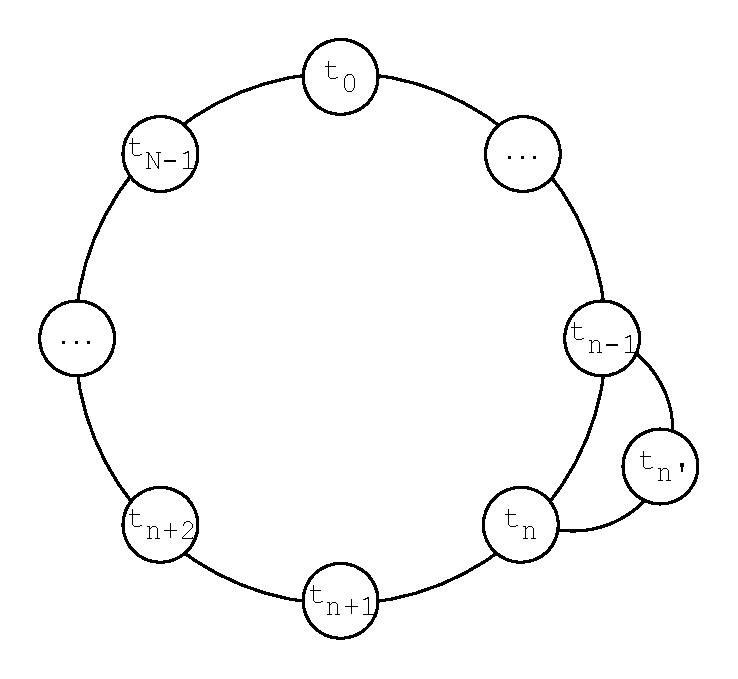
\includegraphics{tokenring-bootstrapping.eps}}
  \end{center}
  \caption{Node $t_{n\prime}$ during bootstrap into token ring}
  \label{fig:bootstrap}
\end{figure}

The approximate fraction of data that will be migrated from node $t_n$ to $t_{n\prime}$ can be calculated as given in equation~\ref{eq:xferfraction}.  This calculation can be used in selecting a token value that achieves specific load balancing goals within the cluster.  For example if a particular node has limited storage, bandwidth, or processing capability, it may make sense to assign it responsibility for a smaller slice of the token range.

A second common way to bootstrap a new node is for the cluster to select a token dictating this nodes placement in the ring. The goal of the election is to choose a token for the new node that will make it responsible for approximately half of the data on the node with the most data that does not already have another node bootstrapping into its range \cite{ref:source,ref:cwiki}.  While this process is technically an election in distributed systems vernacular, nodes are not contacted in an ad-hoc way to initiate this election.  Rather, the new node unilaterally makes this decision based on storage load data gossiped from other nodes periodically \cite{ref:source,ref:cgossip}.

\begin{equation}\label{eq:xferfraction}
\frac{t_{n\prime} - t_{n-1}}{t_n - t_{n-1}}
\end{equation}

\section{Client Access}\label{s:api}

Client interaction with a decentralized distributed system like Cassandra can be challenging.  One of the more obvious problems is for the client to decide which host it will send requests to.  In the case of Cassandra, each node is capable of responding to any client request \cite{ref:cwiki}.  However, choosing a node with a replica of the data to be read or written to will result in reduced communication overhead between nodes to coordinate a response.  It follows that routing all requests to a single client can be the source of bottlenecks in the system. In addition, if that node has failed or is otherwise unreachable, the entire cluster may be perceived as being unavailable.

The Cassandra data store is implemented in Java.  However there is no native Java API for communicating with Cassandra from a separate address space.  Instead Cassandra implements services using \emph{Thrift} \cite{ref:thrift,ref:cwiki}.  Thrift is a framework that includes a high level grammar for defining services, remote objects and types, and a code generator that produces client and server RMI stubs in a variety of languages.  As of this writing, many languages are supported including Java, Ruby, Python, and Erlang.  Each Cassandra node starts a Thrift server exposing services for interacting with data and introspecting information about the cluster.

At this time, the Thrift API to Cassandra exhibits all of the challenges discussed thus far; it leaves open the possibility of a perceived single point of failure and does not intelligently route service invocations to replica nodes.  Because of Thrift's generic nature, it is unlikely these issues will be addressed the future.  On the other hand, \emph{Hector} is a native Java client for Cassandra which has begun to tackle the challenges associated with accessing this decentralized system.  Hector itself is actually a layer on top of the Thrift API and as such it depends on its client and server side bindings \cite{ref:hectorsource}.  It introspects data about the state of the ring in order to determine the endpoint for each host.  This information is then used to implement three modes of client-level failover \cite{ref:hectorsource}.

\begin{description}
  \item[FAIL\_FAST] implements classic behavior of failing a request of the first node contacted is down
  \item[ON\_FAIL\_TRY\_ONE\_NEXT\_AVAILABLE] attempts to contact one more node in the ring before failing
  \item[ON\_FAIL\_TRY\_ALL\_AVAILABLE] will continue to contact nodes, up to all in the cluster, before failing
\end{description}

As of this writing, no client could be found which intelligently routes requests to replica nodes.  Cassandra's Thrift API supports introspection of the token range for each ring \cite{ref:source}, but this would not help in identifying nodes where replicas are located as that would require knowledge of the replica placement strategy discussed in section~\ref{s:replication}.  A truly intelligent client requires up-to-date information regarding replica locations, token ranges, and the availability status of nodes in the cluster.  This being the case, it stands to reason that such a client would need to become a receiver of at least a subset of the gossip passed between nodes and thus an actual member of the cluster.  Depending on an application's purpose, it may make sense to distribute a number of clients throughout the cluster with different responsibilities.  This may also be a strategy for balancing the workload for a number of different clients operating on data retrieved from the Cassandra cluster.  In this style, clients become not passive users of the cluster, but active members of it.  It is expected that best practices for client interaction with Cassandra and similar decentralized data stores will experience significant attention in the near future.

\section{Case Study: Modeling Airline Activity}\label{s:study}

To illustrate the architectural principles discussed this far, this paper attempts to model a problem domain familiar to the audience (or at least the regular traveler).  The largest known users of Cassandra in the industry are social networking sites such as Facebook, Twitter, and Digg \cite{ref:cwiki,ref:diggfuture}.  The most readily available examples of Cassandra usage focus on social networking applications. It is the goal of this paper to contribute to the breadth of examples in the community by studying an unrelated use case--modeling commercial airline activity.  More specifically, a simple study is presented which models airline activity and allows searching for flights from one airport to another with a configurable number of connections.  Following this study, a discussion is held regarding the merits and drawbacks of applying Cassandra to this problem domain. The author has made all source code for data manipulation and search discussed in this section available on github \cite{ref:dfsource} in a project named \emph{Brireme} \footnote[1]{A brireme is a ship used in Ancient Greece during the time of Cassandra}.

In this example we largely ignore the possibilities of inconsistent data that could arise when using an eventually consistent store such as Cassandra.  It is assumed that the likelihood of a user deciding on a flight that will change over the course of their search is acceptably low.  In the event that a particular flight is invalidated over the course of a search, it is assumed that, for example, a purchasing system would alert the user requiring them to begin their search again.  As demonstrated by the CAP Theorem in section~\ref{s:cap}, such risks cannot be completely mitigated when working with changing data at sufficiently large scale.

In order to model airline activity in a way that allows searching for flights on a given day, we must carefully select a data model and system of unique keys supporting required searches.  All examples are in the context of a single keyspace.  Each query will contain four pieces of information: a \emph{date}, \emph{departure airport}, \emph{arrival airport}, and total number of flights allowed, or \emph{hops}.  Because we are interested in following a linked list of flights from the departure airport, a lookup is required that easily finds lists of flights departing an airport on a given day.  For this reason, a \emph{column family} is introduced which we call \emph{FlightDeparture} that, given a key of day and departure airport, provides a listing of flights.  For example, the following map data structure shows an abbreviated list of flights departing Washington Reagan Airport on July 20, 2010.  The key is \emph{20100720-DCA} and the list of flight ids are contained within the value.

\begin{verbatim}
20100720-DCA =>
  (201007200545-DCA-CLT-US-1227,
   201007200545-DCA-MBJ-US-1227,
   201007200600-DCA-ATL-DL-2939,
   201007200600-DCA-ATL-FL-183,
   201007200600-DCA-DCA-DL-6709,
   . . .
   201007200600-DCA-DFW-AA-259)
\end{verbatim}

\noindent
To model this data structure we introduce a new column family named \emph{FlightDeparture}.  The departure date and airport are combined to create a unique key for each row that contains a complete listing of flights.  Each of these flights are represented as single columns within the the row.  Note that the column identifier itself contains all the information this column family is designed to store.  This is by design to limit the amount of data contained in a row and thus helping minimize bandwidth usage and latency during searches.

A separate column family we call \emph{Flight} contains detailed information regarding flights.  The column name of a row in the \emph{FlightDeparture} column family (e.g.\ $201007200730-DCA-SEA-AA-1603$) is a row key which may be used to look up the columns comprising that flight in the \emph{Flight} column family.  The \emph{Flight} column family holds more detailed information regarding a flight in question.

\begin{verbatim}
201007200730-DCA-SEA-AA-1603 =>
  (takeoff,201007200730)  
  (landing,201007201200)
  (flight,1603)         
  (departureCountry,US)   
  (departureCity,WAS)     
  (departureAirport,DCA)  
  (carrier,AA)            
  (arrivalCountry,US)     
  (arrivalCity,SEA)       
  (arrivalAirport,SEA)    
\end{verbatim}

In addition to these primary column families, auxiliary column families \emph{Carrier} and \emph{Airport}, are maintained for looking up further details for a given flight.  The row keys for these column families can be found in the respective columns from rows in the \emph{Flight} column family.  This information could be stored as super columns within a single Flight row, and such de-normalization is often a good strategy for minimizing bandwidth and protocol overhead between the client and nodes in the cluster as it reduces the need to issue additional requests.  Such a strategy trades disk usage for speed of information retrieval which, for a single node, would present storage problems for a sufficiently large number of flights or details regarding the carrier and airports involved.

Source data for this demonstration was obtained from OAG \cite{ref:oag}.  Flight data is given in schedule format which is a compact representation of the flights an airline intends to fly.  This includes the carrier, start day, end day, days of week, departure and arrival airport, and flight number along with other fields not used here.  In order to efficiently search this data for flights on a particular day it must be mapped onto our data model.  The source data is expanded from flight schedules to flight instances and stored in Cassandra.  A small subset of data is chosen for this paper which captures activity at a selection of airports over the course of a few weeks.  Even this small data set represents nearly 22 million flights and 2 gigabytes of source data.  If all data is captured and denormalized to further improve query performance, this data volume can be expected to grow by orders of magnitude.  A similar data set stored in a relational database with secondary indexes necessary for temporal search will be larger still, due to the additional storage requirements and other relational storage overhead.

With future planned flights loaded into Cassandra, an algorithm for searching flights over a number of hops is developed and shown in Appendix~\ref{apx:flightSearchAlgorithm} with a Java implementation given in Appendix~\ref{apx:flightSearchJava} \footnote[1]{The full Java implementation from the author may be found at \cite{ref:dfsource}}.  The procedures $get\_flights\_by\_origin$ and $get\_flight\_by\_id$ are taken to be simple implementations that look up single rows of data using the respective \emph{FlightDeparture} and \emph{Flight} column families using the provided key.

The algorithm given is straightforward to understand and its data access pattern of single object lookups lends itself well to implementation over a key-value store.  In addition, experience running this algorithm shows that, in many cases, flight combinations covering three hops can be calculated in under a minute on a single Cassandra node.  Two-hop flight routes can be calculated in just a few seconds.  The primary latency is the communication overhead involved in making repeated requests for flights and, as long as nodes are connected by high bandwidth cable, it is expected that these algorithms would maintain a similar performance profile as the cluster grows to encompass many nodes.  This hypothesis is made based on the one-hop DHT substrate underlying Cassandra discussed in section~\ref{s:storage}.  Further research is needed to understand how well this model scales with system and data growth.  Were this data modeled in a traditional normalized relational database, a single table would likely be used to represent flight data. Indexes supporting constraints on airport and flight times without full table scans would also need to be in place for efficient queries.  The above algorithm could implement its data access through interaction with a relational database, but such an approach would not scale gracefully as data set growth requires multiple nodes.  As indexes supporting these queries grow ever larger to support larger data sets, partitioning across additional nodes would preset a challenge.  The data designer would be faced with dropping dependencies on database features, such as joins, secondary indexes, and other features that do not scale well to multi-node, multi-master environments.  One approach would be to implement a database schema in which the key for a particular flight, or other piece of information, indicates the node on which it is running.  Such a pattern closely resembles a key-value store like Cassandra but begins to abandon the relational features it was designed for.


\section*{Conclusions}\label{s:conclusion}

This paper has provided an introduction to Cassandra and fundamental distributed systems principles on which it is based.  The concept of distributed hash tables has been discussed both in general and as a substrate for building a decentralized, evolvable key-value data store.  Cassandra's model for trading consistency for availability and latency has been founded by referencing the CAP Theorem and an alternate, lesser-known model known as PACELC.  We have seen how data can be distributed across a wide-area network with intelligent replica placement to maximize availability in the event of node failure and network partitioning.  Throughout this discussion we have contrasted this distributed key-value design with the traditional relational database and provided a formula for working with data at internet scale.  Lastly, an example modeling a real world problem domain with large data requirements has been used to illustrate important principles in this paper.  In doing so, the goal has been to add to the breadth of examples in the community for working with sparse column data stores like Cassandra.

\newpage

\appendix
\section{Flight Search Algorithm}\label{apx:flightSearchAlgorithm}
\begin{@twocolumnfalse}
\begin{program}
\BEGIN %
  \mbox{Algorithm for finding flights over a given number of hops}
  \PROC |get_flights|(date,dep\_airport,dest\_airport,hops) \BODY
    options = ();
    legs = ();
    \COMMENT{get all flights leaving $airport$};
    \COMMENT{on $date$ using $FlightDeparture$ CF};
    flight\_keys := get\_flights\_by\_origin(concat(date,airport));
    \FOR flight\_keys.each() \Rightarrow |flight\_key| \DO
      arr\_airport := get\_arr\_airport(flight\_key);
      \IF arr\_airport = dep\_airport
        \COMMENT {capture this one hop flight};
        options.add(get\_flight\_by\_id(flight\_key));
      \ELSIF hops > 1
        \COMMENT {look up flight details from the Flight CF};
        flight := get\_flight\_by\_id(flight\_key);
        \COMMENT{recursively search for flights over};
        \COMMENT{the requested number of hops};
        legs.push(flight);
        traverse\_flights(options,legs,date,dest\_airport,2,hops);
        legs.pop();
      \FI
    \OD
    \COMMENT{Return a list of flight routes matching};
    \COMMENT{our criteria. Each element of this list};
    \COMMENT{is a list of connecting flights from};
    \COMMENT{dep\_airport to dest\_airport}
    return(options);
  \ENDPROC
  
  \mbox{recursive portion of algorithm}
  \mbox{performs a depth-first traversal of flight options}
  \PROC |traverse\_flights|(options,legs,date,dest\_airport,level,hops) \BODY
    last\_leg := legs.peek();
    arrival := last\_leg.arrival\_airport();
    flight\_keys := get\_flights\_by\_origin(concat(date,arrival));    
    \FOR flight\_keys.each() \Rightarrow |flight\_key| \DO
      flight := get\_flight\_by\_id(flight\_key);
      \COMMENT{see if flight is to destination airport and departs};
      \COMMENT{after the last leg lands at connecting airport};
      \IF flight.happens\_after(last\_leg)
        \IF arrival = dest\_airport
          route = ();
          route.add\_all(legs);
          route.add(flight);
          options.add(route);
        \ELSE
          \IF level < hops
          legs.push(flight);
          traverse\_flights(
            options,legs,date,dest\_airport,
            level+1,hops);
          legs.pop();
          \FI
        \FI
      \FI
    \OD
  \ENDPROC
\END
\end{program}

\newpage

\section{Flight Search Algorithm (Java Implementation)}\label{apx:flightSearchJava}

\begin{verbatim}
List<List<FlightInstance>> getFlights(String day, String dep, String dest,
                                      boolean sameCarrier, int hops) throws Exception {
    
  // holds all verified routes
  List<List<FlightInstance>> options = new ArrayList<List<FlightInstance>>();
  
  // temporary data structure for passing connecting information
  Stack<FlightInstance> legs = new Stack<FlightInstance>();
  
  List<String> flightIds = getFlights(day, dep);
  for (String flightId : flightIds) {
    String arrivalAirport = getArrivalAirport(flightId);
    if(arrivalAirport.equals(dest)) {
      // build new connection list with only this flight
      List<FlightInstance> flights = new ArrayList<FlightInstance>();
      flights.add(getFlightById(flightId));
      options.add(flights);
    }
    else if(hops > 1) {
      // look at possible destinations connecting from this flight
      legs.push(getFlightById(flightId));
      traverseFlights(options, legs, day, dest, sameCarrier, 2, hops);
      legs.pop();
    }
  }
  return options;
}

void traverseFlights(List<List<FlightInstance>> optionList,
                     Stack<FlightInstance> legs,
                     String day, String arr,
                     boolean sameCarrier, int level, int hops) throws Exception {

  // get the connection information from the last flight and
  // search all outbound flights in search of our ultimate destination
  FlightInstance lastLeg = legs.get(legs.size()-1);
  String arrivingAt = lastLeg.getArrivalAirport();
  List<String> flightIds = getFlights(day, arrivingAt);
  for (String flightId : flightIds) {
    FlightInstance flight = getFlightById(flightId);
    if(flight.happensAfter(lastLeg)) {
      if (canTerminate(flight,arr,sameCarrier,lastLeg)) {
        // build new route with all prior legs, adding this flight to the end
        List<FlightInstance> route = new ArrayList<FlightInstance>(legs.size()+1);
        route.addAll(legs);
        route.add(flight);
        // copy this route to the verified set that go from dep -> arr
        optionList.add(route);
      }
      else if (level < hops) {
        legs.push(flight);
        traverseFlights(optionList,legs,day,arr,sameCarrier,level+1,hops);
        legs.pop();
      }
    }
  }
}

boolean canTerminate(FlightInstance flight,
                     String arr, boolean sameCarrier,
                     FlightInstance lastLeg) {
  return flight.getArrivalAirport().equals(arr) &&
         (!sameCarrier || flight.hasSameCarrier(lastLeg));
}
\end{verbatim}

\newpage

\end{@twocolumnfalse}

\begin{thebibliography} {99}
\bibitem{ref:source} Misc.~Authors {\sl Apache Cassandra 0.6.3 Java Source Code} Available from http://cassandra.apache.org
\bibitem{ref:bigtable} F.~Chang, J.~Dean, S.~Ghemawat, W.~C.~Hsieh, D.~A.~Wallach, M.~Burrows, T.~Chandra, A.~Fikes, and R.~E.~Gruber, {\sl Bigtable: A Distributed Storage System for Structured Data} OSDI'06: Seventh Symposium on Operating System Design and Implementation, 2006, Seattle,~WA,~2006.
\bibitem{ref:dynamo} G.~DeCandia, D.~Hastorun, M.~Jampani, G.~Kakulapati, A.~Lakshman, A.~Pilchin, S.~Sivasubramanian, P.~Vosshall, and W.~Vogels, {\sl Dynamo: Amazon’s Highly Available Key-value Store} In Proceedings of twenty-first ACM SIGOPS symposium on Operating systems principles (2007), ACM Press New York,~NY,~USA, pp.~205–220
\bibitem{ref:facebook} A.~Lakshman, P.~Malik, {\sl Cassandra - A Decentralized Structured Storage System}, Cornell, 2009
\bibitem{ref:thrift} M.~Slee, A.~Agarwal, M.~Kwiatkowski, {\sl Thrift: Scalable Cross-Language Services Implementation} Facebook, Palo Alto,~CA,~2007
\bibitem{ref:hector} R.~Tavory, {\sl Hector – a Java Cassandra client} http://prettyprint.me/2010/02/23/hector-a-java-cassandra-client February,~2010
\bibitem{ref:hectorsource} R.~Tavory, {\sl Hector Java Source Code} Available from http://github.com/rantav/hector
\bibitem{ref:twiki} {\sl Thrift Wiki} http://wiki.apache.org/thrift
\bibitem{ref:fault} F.~Cristian, {\sl Understanding Fault-Tolerant Distributed Systems} University of California, San Diego, La Jolla, CA, May~1993
\bibitem{ref:onehop} A.~Gupta, B.~Liskov, and R.~Rodrigues, {\sl Efficient Routing for Peer-to-Peer Overlays}, Proceedings of the 1st Symposium on Networked Systems Design and Implementation, MIT Computer Science and Artificial Intelligence Laboratory, 2004
\bibitem{ref:brewer} N.~Lynch, S.~Gilbert, {Brewer's Conjecture and the Feasibility of Consistent, Available, Partition-Tolerant Web Services} ACM SIGACT News, v. 33 issue 2, 2002, p. 51-59.
\bibitem{ref:pacelc} D.~Abdi, {\sl Problems with CAP, and Yahoo's little known NoSQL system} http://dbmsmusings.blogspot.com/2010/04/problems-with-cap-and-yahoos-little.html, Yale~University, April,~2010
\bibitem{ref:chord} I.~Stoica, R.~Morris, D.~Liben-Nowell, D.~Karger, M.~F.~Kaashoek, F.~Dabek, and H.~Balakrishnan, {\sl Chord: A scalable peer-to-peer lookup service for internet applications} Technical report, MIT LCS, 2002
\bibitem{ref:beyondnap}K.~Nagaraja, S.~Rollins, M.~Khambatti, {\sl Looking Beyond the Legacy of Napster and Gnutella}
\bibitem{ref:cwiki} J.~Ellis, et. al., {\sl Cassandra Wiki} http://wiki.apache.org/cassandra/FrontPage, 2010
\bibitem{ref:cgossip} J.~Ellis, et. al., {\sl Cassandra Gossiper Architecture} http://wiki.apache.org/cassandra/ArchitectureGossip, 2010
\bibitem{ref:dht} {\sl Distributed Hash Table} http://en.wikipedia.org/wiki/Distributed\_hash\_table
\bibitem{ref:md5} {\sl MD5} http://en.wikipedia.org/wiki/MD5
\bibitem{ref:datascience} M.~Loukides, {\sl What is data science? Analysis: The future belongs to the companies and people that turn data into products.} http://radar.oreilly.com/2010/06/what-is-data-science.html, June 2010
\bibitem{ref:asfl} Apache Software Foundation, {\sl Apache License Version 2.0}  http://www.apache.org/licenses/, January,~2004
\bibitem{ref:dbsharding} J.~Peryn, {\sl Database Sharding at Netlog} Presented at FOSDEM 2009, Brussels,~Belgium, February,~2009
\bibitem{ref:apacheblog} Apache Software Foundation, {\sl The Apache Software Foundation Announces New Top-Level Projects} https://blogs.apache.org/foundation/entry/the\_apache\_software\_foundation\_announces4, Forest Hill,~MD, May~4,~2010
\bibitem{ref:diggfuture} I.~Eure, {Looking to the future with Cassandra} http://about.digg.com/blog/looking-future-cassandra, September,~2009
\bibitem{ref:oag} OAG Aviation http://www.oag.com/
\bibitem{ref:cdk} G.~Coulouris, J.~Dollimore, T.~Kindberg, {\sl Distributed Systems: Concepts and Design} Addison Wesley, 2005
\bibitem{ref:dfsource} D.~Featherston (the author) {\sl Brireme project on Github} http://github.com/dietrichf/brireme
\end{thebibliography}

\end{document}
